
\documentclass[12pt]{article}
\usepackage[a4paper, margin=.30in]{geometry}
\usepackage{graphicx ,
            wrapfig,
            xcolor, 
            enumerate,
            amsmath,
			fontenc,
			tcolorbox
            }

\newcommand\headerMe[2]{\noindent{}#1\hfill#2}
\renewcommand{\thesection}{\Roman{section}}

\author{Zakaria HAOUZAN}
\date{\today}

\begin{document}
% headers --------------
\headerMe{Matière : Physique-Chimie}{Professeur : Zakaria HAOUZAN}\\
\headerMe{Unité : Transformations nucléaires }{Établissement : Lycée SKHOR qualifiant}\\
\headerMe{Niveau : 2BAC-SM-X}{Heure : 10H}\\

% ------Content ________
\begin{center}

    \Large{Leçon $N^{\circ} 4 $: \color{red}Noyau , énergie et masse }
\end{center}

%\begin{wrapfigure}[10]{r}{0.5\textwidth}
%    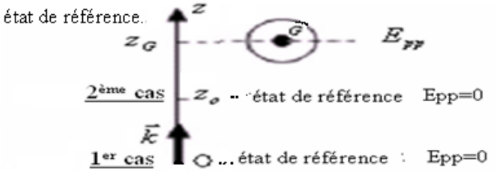
\includegraphics[width=0.5\textwidth]{./img/img00.png}
%\end{wrapfigure}


\section{ Equivalence : Masse - Energie  }

\subsection{La relation Albert Einstein:  }
En 1905 Albert Einstein postulat l'équivalence entre la masse et l'énergie suivante :
\emph{Tout corps de masse "m" au repos, possède une énergie égale au produit de sa masse par le carré de la vitesse
de la lumière  dans le vide.}$$E = m.c^2$$
\begin{itemize}
	\item E : s'appelle l'énergie massique. (J)
	\item m: la masse du corps au repos. (kg)
	\item c: vitesse se la lumière dans le vide $c=3.10^8m/s$
	\end{itemize}
	Cette relation montre que toute variation de masse $\Delta{m}$ d'un système s'accompagne d'une variation d'énergie
	$\Delta{E}=\Delta{m}.c^2$
	\subsection{Unités de masse et d'énergie: }
	\subsubsection{ Unité de masse atomique (uma)- (u)}
En physique nucléaire, l'unité convenable de la masse s'appelle unité de masse
atomique symbolisée par u, elle représente $\frac{1}{12}$ 12
de la masse d'un atome du carbone $_6^{12}C$.
$$1uma = \frac{m(_6^{12}C)}{12} = \frac{M(_6^{12}C)}{12N_a} = 1,66.10^{-27}Kg$$

avec : $N_a = 6,02.10^{23} mol$ le nombre d'Avogadro ;$M(_6^{12}C) = 12/mol$ masse molaire du carbone

$m_p = 1,0073u$ masse d'un proton ; $m_n = 1,0087 u$

\subsubsection{Unité de l’énergie : Electronvolt}
En physique nucléaire, l'unité convenable de l'énergie est électronvolt et ces
multiples comme mégaélectronvolt MeV : $1ev = 1,6.10^{-19}J$ ; $1Mev = 1,6.10^{-13}J$
\subsubsection{ Energie équivalente à l'unité de masse atomique : }
D'après la relation d'Albert Einstein et pour la masse égale à 1 u on a
$E = m.c^2 = 1,66054.10^{-27}.(299792458)^2 = 1492,42.10^{-13}J$

donc : $E = \frac{1492.10^{-13}}{1,602177.10^{-13}}$ = 931,5 Mev.
$$1uma = 931,5 Mev/c^2$$

\begin{tcolorbox}
	Exercice d’application N°1: Calculer l’énergie de masse relative à un proton en SI puis en Mev. Données : $m_p = 1,6726.10^{-27} kg$
\end{tcolorbox}

\section{Energie de liaison d'un noyau : }
\subsection{Défaut de masse : }

\begin{wrapfigure}[1]{r}{0.2\textwidth}
	\vspace{-0.9cm}
	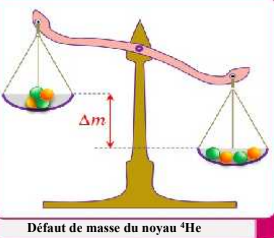
\includegraphics[width=0.2\textwidth]{./img/defautMasse.png}
\end{wrapfigure}


Le défaut de masse d'un noyau de
symbole $_Z^AX$ est la différence entre la masse des nucléons isolé et au repos est la
masse du noyau au repos, on le symbolise
par :

$$\Delta{m} = Z.m_p + (A-Z).m_n - m(_Z^AX)$$
Le défaut de masse est toujours strictement positif.
\begin{tcolorbox}
	Exercice d’application N°2:

	Calculer, en u et en kg, le défaut de masse du noyau du carbone $^7_3Li$

	On donne : $m_P = 1,0073 u$ ; $m_N = 1,0087 u$ ; $m( ^7Li) = 7,0160 u$ et $1u=1,66.10^{-27} kg$.
\end{tcolorbox}
\subsection{Energie de liaison:}
\subsubsection{ Définition :}
L'énergie de liaison d'un noyau noté $E_l$ est l'énergie qu'il faut apporter à un noyau au
repos pour le dissocier en ses nucléons " protons et neutrons " isolés et au repos :
$$_z^AX \rightarrow Z._1^1p + (A-Z)_0^1n$$

On l'exprime par la relation: $$E_l = \Delta{m}.C^2 = [Z.m_p + (A-Z).m_n - m(_z^AX)]$$
avec $\Delta{m}$ est défaut de masse. L'unité de l'énergie de liaison est MeV
\begin{center}
	%\vspace{-0.9cm}
	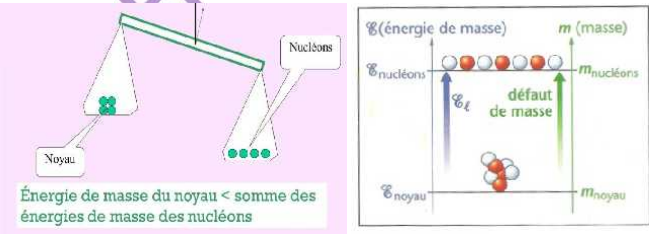
\includegraphics[width=0.6\textwidth]{./img/energieLaison.png}
\end{center}
\begin{tcolorbox}
	Exercice d’application N°3:

	Calculer, en Mev, l’énergie de liaison du noyau du carbone $^7_3Li$
\end{tcolorbox}

\subsubsection{Energie de liaison par nucléon : }
L'énergie de liaison par nucléon est définit par la relation : $E = \frac{E_l}{A}$
l'unité est MeV/nucléon.
\begin{tcolorbox}
	Exercice d’application N°4:

	Calculer, en Mev/nucléon, l’énergie de liaison du noyau du carbone $^7_3Li$
\end{tcolorbox}

\subsubsection{la stabilité des noyaux radioactifs: }
A partir de l’énergie de liaison par nucléon, on peut comparer la stabilité de 2
noyaux radioactifs

Plus l'énergie de liaison par nucléon est grande plus le noyau est stable.

$$\frac{E_l(X_1)}{A_1} \geq \frac{E_l(X_2)}{A_2}$$

X1 est plus stable que X2

Plus l'énergie de liaison par nucléon est grande plus la désintégration
du noyau radioactif est difficile et donc plus le noyau est stable.

\subsection{Courbe d'Aston: }

La courbe d'Aston représente l'opposé de l'énergie de liaison par nucléon $-\frac{E_l}{A}$ en fonction du nombre de nucléon A, il permet de comparer la stabilité des différents
noyaux.
\begin{wrapfigure}[11]{r}{0.44\textwidth}
	%\vspace{-0.9cm}
	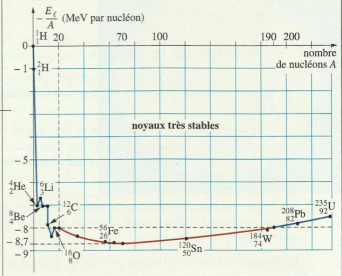
\includegraphics[width=0.44\textwidth]{./img/aston.png}
\end{wrapfigure}
\begin{itemize}
	\item Pour $20 \leq A \leq 190$ on constate sure la courbe des valeurs minimales de  $-\frac{E_l}{A}$ sa valeur absolue $leq 8$MeV/nucléon cette partie contient les noyaux les plus stable.
	\item $A \leq 20 $et $A \geq 190$ l'énergie de liaison par nucléon de ces noyaux est faible,
c'est pour cela ces noyaux sont instable. Ils peuvent se transformer aux noyaux plus
stables selon deux types de réactions nucléaires : 

\item Pour les noyaux lourds $(A \geq 190)$ instables, chaque noyau est scindé en deux noyaux
plus légers, on appelle ce phénomène la fission nucléaire.

\item Pour les noyaux légers $(A \leq 20)$ ils se fusionnent entre eux pour former un noyau
plus lourd, on appelle ce phénomène la fusion nucléaire.
\end{itemize}

\section{Fission et fusion nucléaire : }

La fission nucléaire et la fusion nucléaire sont des transformations nucléaires
forcées ou provoquées c.à.d nécessitant un apport d’énergie de l’extérieure.

\subsection{ La Fission nucléaire :  }
\begin{wrapfigure}[1]{r}{0.34\textwidth}
	\vspace{-1cm}
	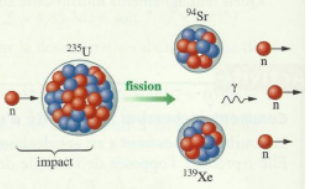
\includegraphics[width=0.34\textwidth]{./img/fission.png}
\end{wrapfigure}
La fission est une réaction nucléaire dont laquelle un noyau lourd 

$A\geq190$ est
scindé, sous l’impact d’un neutron, en deux noyaux plus légers.

Exemple : l’envoie un neutron libères sur un noyau d’Uranium :
$$ _{92}^{235}U + _0^1n \rightarrow _{36}^94Kr + _{56}^{139}Ba + 2_0^1n$$

Remarque :

 Chacun des 2 neutrons libères va provoquer, à son tour, la fission d’un atome
d’uranium et ainsi de suite : on parle de réaction en chaine.

\subsection{La Fusion nucléaire : }

\begin{wrapfigure}[11]{r}{0.3\textwidth}
	\vspace{-2cm}
	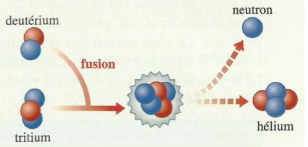
\includegraphics[width=0.3\textwidth]{./img/fussion.png}
	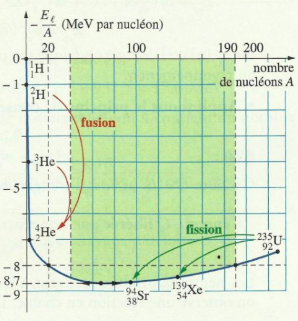
\includegraphics[width=0.3\textwidth]{./img/stone_fisson.png}
\end{wrapfigure}



Deux noyaux légers $A \leq 20$ fusionnent pour donner naissance à un noyau plus
lourd stable. 

Exemple 1: Dans le soleil le noyau d'hydrogène fusionne pour former de l'hélium.

$$4_1^1H \rightarrow _2^4He + 2_1^0e$$

Ce type de réaction rarement produite c’est la bombe H .Elle a lieu naturellement
dans le soleil et les étoiles. Les scientifiques travaillent pour la contrôler "  projet
ITER  " car elle produit 4 fois plus d’énergie que la fission nucléaire

\section{Le bilan massique et énergétique d'une réaction nucléaire : }

\subsection{Variation de masse et d’énergie :}
\begin{wrapfigure}[5]{r}{0.44\textwidth}
	%\vspace{-0.9cm}
	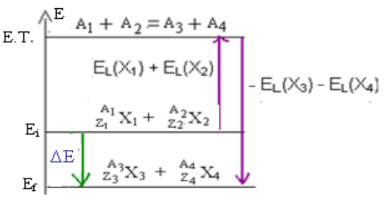
\includegraphics[width=0.44\textwidth]{./img/diag_00.png}
\end{wrapfigure}


On considère la réaction nucléaire suivante :
$$_{z_1}^{A_1}X_1 + _{z_2}^{A_2}X_2 \rightarrow _{z_3}^{A_3}X_3 + _{z_4}^{A_4}X_4 $$
Avec X le symbole du noyau 

\begin{itemize}
	\item Le bilan massique : $\Delta{m} = m_{produits} - m_{reactifs}$
	\item $\Delta{m} = (m(X_4) + m(X_3))- (m(X_2) + m(X_1)) $
	\item Le bilan énergétique $\Delta{E} $: 
		$$\Delta{E} = \Delta{m}.C^2=[(m(X_4) + m(X_3))- (m(X_2) + m(X_1))].C^2$$
	\item L'énergie de cette transformation est donnée par la relation suivante:
		$$\Delta{E} = [(E_l(X_1) + E_l(X_2))- (E_l(X_3) + E_l(X_4))]$$
	\item Si $\Delta{E} \leq 0$la réaction est exothermique.
	\item Si $\Delta{E} \geq 0$la réaction est endothermique.
	\item L’énergie libérer par cette transformation : $E_{lib} = \Delta{E}$
\end{itemize}

\section{Bilan énergétique des transformations nucléaires spontanées:}
\subsection{Bilan énergétique de la transformation $\alpha$ : }
\begin{wrapfigure}[5]{r}{0.24\textwidth}
	\vspace{-1.2cm}
	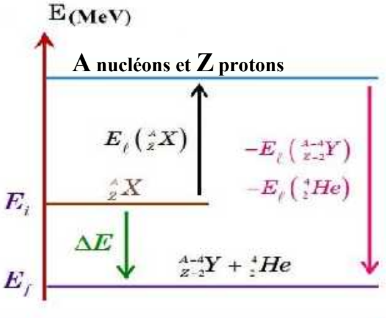
\includegraphics[width=0.24\textwidth]{./img/diag_alpha.png}
\end{wrapfigure}


Equation de désintégration $\alpha$ : $_z^AX \rightarrow _{z-2}^{A-4}Y + _2^4He$

Bilan énergétique : $\Delta{E} =[(m(_{z-2}^{A-4}Y) + m(_2^4He))- (m(_z^AX) ].C^2 \leq 0 $

\subsection{Bilan énergétique de la transformation $\beta^-$ : }

\begin{wrapfigure}[5]{r}{0.24\textwidth}
	\vspace{-1.2cm}
	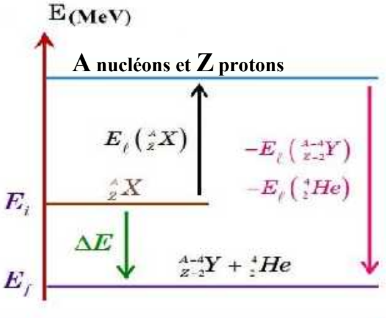
\includegraphics[width=0.24\textwidth]{./img/diag_alpha.png}
\end{wrapfigure}


Equation de désintégration $\beta^-$ : $_z^AX \rightarrow _{z+1}^{A}Y + _{-1}^0e$

Bilan énergétique : $\Delta{E} =[(m(_{z+1}^{A}Y) + m(_{-1}^0e))- (m(_z^AX) ].C^2 \leq 0 $

\section{Les effets biologiques de la radioactivité:}

Les rayonnements alpha, bêta et gamma constituent un danger pour l’homme car ce sont des rayonnements
ionisants. La gravité des effets biologiques de la radioactivité dépend du type de radiation et de la dose absorbée par
l'organe touché. Cependant la radioactivité est présente partout et elle trouve des applications dans de nombreux
domaines aujourd’hui, notamment dans le domaine médical mais en faibles doses.





%wfg---------------------------------------------------------------sf 
%\begin{center}
   %\begin{tabular}{ |c|c|c|c|c|c|c| }
      %\hline
      %km & hm & dam & \bf{m} & dm & cm & mm \\
      %\hline
        %&   &    &  &   &   & \\
%\hline
%\end{tabular}
%On place un seul nombre dans chaque case.
%\end{center}
%\begin{center}
   %\begin{tabular}{ |c|c|c|c|c|c|c| }
      %\hline
      %$km^2$ & $hm^2$ & $dam^2$ & \bf{$m^2$} & $dm^2$ & $cm^2$ & $mm^2$ \\
      %\hline
        %&   &    &  &   &   & \\
%\hline
%\end{tabular}
%\end{center}


\end{document}

